\documentclass[doc]{apa6}
\usepackage{lmodern}
\usepackage{amssymb,amsmath}
\usepackage{ifxetex,ifluatex}
\usepackage{fixltx2e} % provides \textsubscript
\ifnum 0\ifxetex 1\fi\ifluatex 1\fi=0 % if pdftex
  \usepackage[T1]{fontenc}
  \usepackage[utf8]{inputenc}
\else % if luatex or xelatex
  \ifxetex
    \usepackage{mathspec}
  \else
    \usepackage{fontspec}
  \fi
  \defaultfontfeatures{Ligatures=TeX,Scale=MatchLowercase}
\fi
% use upquote if available, for straight quotes in verbatim environments
\IfFileExists{upquote.sty}{\usepackage{upquote}}{}
% use microtype if available
\IfFileExists{microtype.sty}{%
\usepackage{microtype}
\UseMicrotypeSet[protrusion]{basicmath} % disable protrusion for tt fonts
}{}
\usepackage{hyperref}
\hypersetup{unicode=true,
            pdftitle={Between the devil and the deep blue sea: Tensions between scientific judgement and statistical model selection},
            pdfauthor={Danielle J. Navarro},
            pdfkeywords={model selection; science; statistics},
            pdfborder={0 0 0},
            breaklinks=true}
\urlstyle{same}  % don't use monospace font for urls
\usepackage{graphicx,grffile}
\makeatletter
\def\maxwidth{\ifdim\Gin@nat@width>\linewidth\linewidth\else\Gin@nat@width\fi}
\def\maxheight{\ifdim\Gin@nat@height>\textheight\textheight\else\Gin@nat@height\fi}
\makeatother
% Scale images if necessary, so that they will not overflow the page
% margins by default, and it is still possible to overwrite the defaults
% using explicit options in \includegraphics[width, height, ...]{}
\setkeys{Gin}{width=\maxwidth,height=\maxheight,keepaspectratio}
\IfFileExists{parskip.sty}{%
\usepackage{parskip}
}{% else
\setlength{\parindent}{0pt}
\setlength{\parskip}{6pt plus 2pt minus 1pt}
}
\setlength{\emergencystretch}{3em}  % prevent overfull lines
\providecommand{\tightlist}{%
  \setlength{\itemsep}{0pt}\setlength{\parskip}{0pt}}
\setcounter{secnumdepth}{0}
% Redefines (sub)paragraphs to behave more like sections
\ifx\paragraph\undefined\else
\let\oldparagraph\paragraph
\renewcommand{\paragraph}[1]{\oldparagraph{#1}\mbox{}}
\fi
\ifx\subparagraph\undefined\else
\let\oldsubparagraph\subparagraph
\renewcommand{\subparagraph}[1]{\oldsubparagraph{#1}\mbox{}}
\fi

%%% Use protect on footnotes to avoid problems with footnotes in titles
\let\rmarkdownfootnote\footnote%
\def\footnote{\protect\rmarkdownfootnote}


  \title{Between the devil and the deep blue sea: Tensions between scientific
judgement and statistical model selection}
    \author{Danielle J. Navarro\textsuperscript{1}}
    \date{}
  
\shorttitle{Science and statistics}
\affiliation{
\vspace{0.5cm}
\textsuperscript{1} University of New South Wales}
\keywords{model selection, science, statistics}
\usepackage{csquotes}
\usepackage{upgreek}
\captionsetup{font=singlespacing,justification=justified}

\usepackage{longtable}
\usepackage{lscape}
\usepackage{multirow}
\usepackage{tabularx}
\usepackage[flushleft]{threeparttable}
\usepackage{threeparttablex}

\newenvironment{lltable}{\begin{landscape}\begin{center}\begin{ThreePartTable}}{\end{ThreePartTable}\end{center}\end{landscape}}

\makeatletter
\newcommand\LastLTentrywidth{1em}
\newlength\longtablewidth
\setlength{\longtablewidth}{1in}
\newcommand{\getlongtablewidth}{\begingroup \ifcsname LT@\roman{LT@tables}\endcsname \global\longtablewidth=0pt \renewcommand{\LT@entry}[2]{\global\advance\longtablewidth by ##2\relax\gdef\LastLTentrywidth{##2}}\@nameuse{LT@\roman{LT@tables}} \fi \endgroup}


\usepackage{lineno}

\linenumbers

\authornote{I am grateful to many people for helpful
conversations and comments that shaped this paper, most notably Nancy
Briggs, Berna Devezer, Chris Donkin, Olivia Guest, Daniel Simpson, Iris
van Rooij and Fred Westbrook.

Correspondence concerning this article should be addressed to Danielle
J. Navarro, School of Psychology, University of New South Wales.
Kensington NSW 2052, Sydney, Australia. E-mail:
\href{mailto:d.navarro@unsw.edu.au}{\nolinkurl{d.navarro@unsw.edu.au}}}

\abstract{
Discussions of model selection in the psychological literature typically
frame the issues as a question of statistical inference, with the goal
being to determine which model makes the best predictions about data.
Within this setting, advocates of leave-one-out cross-validation and
Bayes factors disagree on precisely which prediction problem model
selection questions should aim to answer. In this comment, I discuss
some of these issues from a scientific perspective. What goal does model
selection serve when all models are known to be systematically wrong?
How might ``toy problems'' tell a misleading story? How does the
scientific goal of explanation align with (or differ from) traditional
statistical concerns? I do not offer answers to these questions, but
hope to highlight the reasons why psychological researchers cannot avoid
asking them.


}

\usepackage{amsthm}
\newtheorem{theorem}{Theorem}[section]
\newtheorem{lemma}{Lemma}[section]
\theoremstyle{definition}
\newtheorem{definition}{Definition}[section]
\newtheorem{corollary}{Corollary}[section]
\newtheorem{proposition}{Proposition}[section]
\theoremstyle{definition}
\newtheorem{example}{Example}[section]
\theoremstyle{definition}
\newtheorem{exercise}{Exercise}[section]
\theoremstyle{remark}
\newtheorem*{remark}{Remark}
\newtheorem*{solution}{Solution}
\begin{document}
\maketitle

Model selection seems to be an evergreen topic in mathematical
psychology. Given two or more competing theories about the world, each
instantiated as parameterised computational models that provide
different accounts of a data set, how should we decide which model is
better supported by the data? Typically we formulate this as a
statistical inference problem, with various authors arguing for Bayes
factors (e.g., Wagenmakers 2007), minimum description length (e.g.,
Grünwald 2007), cross-validation (e.g., Browne 2000) and a variety of
other possibilities besides. To highlight the behaviour of different
model selection methods, we often consider \enquote{toy problems},
simplified versions of serious inferential scenarios designed to elicit
different intuitions about whether the model selection procedure behaves
sensibly. The large-sample results presented by Gronau and Wagenmakers
(2018) fall within this tradition, highlighted by the Dennis Lindley
quote that motivates the work. The results are perhaps unsurprising
given the known inconsistency of orthodox cross-validation estimators
(Shao 1993), but there is value in highlighting the issue to a broader
audience and noting that a Bayesian formulation does not remove this
limitation. To the extent that some psychologists are unaware of the
need for care when using cross-validation methods -- as indeed they may
be unaware of a need for caution with respect to Bayes factors or any
other model selection procedure -- the paper strikes me as helpful and
timely.

As much as I enjoyed the paper, I wonder whether the simplicity of
exposition comes at a cost. As Vehtari, Simpson, Yau and Gelman (2018)
note in their commentary, Gronau and Wagenmakers' examples apply
leave-one-out cross-validation in a fashion that is rather at odds with
how its advocates recommend that it be used. The original paper
constitutes a strong argument against naive or accidental misuse of some
cross-validation procedures, but the implications for best practice seem
much less obvious. Noting that other commenters have discussed technical
issues in detail, my goal in this paper is to take a slightly broader
view on the tensions between scientific judgement and statistical model
selection.

\subsection{Mistaking the map for the
territory}\label{mistaking-the-map-for-the-territory}

The quote by Lindley asks us to consider the question \enquote{if you
can't do simple problems, how can you do complicated ones?} While I
understand and sympathise with the sentiment, for my own part I would be
tempted to reverse the warning: if we \emph{only} solve simple problems,
we may never learn how to think about the complex ones. As someone who
has tried to use many different model selection tools over the years, I
am of the view that the behaviour of a selection procedure applied to
toy problems is a poor proxy for the inferential problems facing
scientists. As such, if we are to motivate our approach to model
selection by quoting famous statisticians, my preference would be to
start with George Box's (1976, p 792) comment on the dangers of
selective worrying:

\begin{quote}
Since all models are wrong the scientist must be alert to what is
importantly wrong. It is inappropriate to be concerned about mice when
there are tigers abroad.
\end{quote}

\noindent
Everyone who develops model selection tools is of course aware that all
models are wrong. Scientists do not fully understand the phenomena we
are studying (else why study them?) and every formal model-based
description of the phenomenon is wrong in an unknown, systematic
fashion. One consequence of this, I think, is that while it is usually
easy to construct artificial scenarios in which any given procedure
misbehaves, it is often difficult to know what implications they might
have for the real world scientific problems they approximate.

To illustrate how easy it is to tell a misleading story, consider the
behaviour of the Bayes factor -- a procedure I presume Gronau and
Wagenmakers would endorse as sensible -- when presented with a minor
variation of their Example 1. In this scenario there are two models, a
\enquote{general law} \(\mathcal{M}_1\) which asserts that a Bernouilli
probability \(\theta\) equals 1; and an \enquote{unknown quantity} model
\(\mathcal{M}_2\) that expresses uncertainty by placing a uniform
Beta(1,1) prior over \(\theta\). Given a sample \(n\) successes (i.e.,
all observations are 1) the Bayes factor will select \(\mathcal{M}_1\)
with certainty as \(n \rightarrow \infty\), and the variant of
leave-one-out cross-validation they discuss does not. The behaviour of
the Bayes factor seems desirable insofar as \(\mathcal{M}_1\) is the
true model in this scenario. However, it is not difficult to reverse
this intuition and construct an example where this same certainty seems
\emph{un}desirable.

Consider the \enquote{negligible error} scenario in which
\(\mathcal{M}_1\) is \emph{almost} correct: the general law holds, apart
from a single failure. The probability of success is 1, in the sense
that one failure (or indeed any finite number of failures) in an
infinite sequence of successes forms a set of measure zero. The true
probability of success in a frequentist sense is
\(\lim_{n\rightarrow\infty} (n-1)/n = 1\), and similarly, the posterior
expected value of \(\theta\) for the unknown quantity model
\(\mathcal{M}_2\) converges on \(\theta = 1\) in the large sample limit.
In any sense that a pragmatic scientist would care about, the general
law would count as the \enquote{correct} account for the
phenomenon.\footnote{While there are many people who assert that
  \enquote{a single failure is enough to falsify a theory}, I confess I
  have not yet encountered anyone willing to truly follow this principle
  in real life.} Nevertheless the general law model \(\mathcal{M}_1\)
does not have support at the data \(\bm{x}\). So while
\(P(\bm{x}|\mathcal{M}_1)=0\) for all \(n\) after the single failure has
occurred, \(\mathcal{M}_2\) assigns positive prior probability to the
data \[
P(\bm{x}|\mathcal{M}_2) = \int_0^1 \theta^{n-1} (1-\theta) d\theta = B(n,2) = \frac{(n-1)! 1!}{(n+1)!} = (n(n+1))^{-1}
\] The Bayes factor
\(P(\bm{x}|\mathcal{M}_1) / P(\bm{x}|\mathcal{M}_2)\) is therefore 0,
and selects \emph{against} the general law \(\mathcal{M}_1\) with
certainty even though \(\mathcal{M}_1\) makes an \enquote{almost exactly
true} prior prediction, whereas \(\mathcal{M}_2\) assigns the same
degree of prior belief to the true rule \(\theta=1\) as it does to the
exact opposite rule, \(\theta = 0\).

To a statistician the reason for this misbehaviour is obvious, and
rather boring: a general law formulated as a model that does not
accommodate measurement error (and therefore lacks support across most
of the sample space) will behave poorly in a world such as our own that
actually does have such errors. The fact that the Bayes factor produces
counterintuitive inferences when asked to choose between extremely bad
models is not \emph{prima facie} evidence that we should discard Bayes
factors. Rather, it requires that we recognise that Bayes factors can
produce strange answers when none of the models are \enquote{true}. In
this instance the problem arises because the large sample behaviour of
the Bayes factor is to select the model whose prior predictive
distribution \(P(\bm{x}|\mathcal{M})\) is closest in Kullback-Leibler
divergence to the true data generating mechanism,\footnote{For instance,
  Gelman, Carlin, Stern \& Rubin (2004, p586-587) present an analogous
  convergence result for the posterior distribution \(P(\theta|x)\)
  within a single model \(\mathcal{M}\). The result generalises to the
  Bayes factor by noting that the Bayes factor identifies a model with
  the prior predictive distribution \(P(x | \mathcal{M})\). Substituting
  \(P(x | \mathcal{M})\) for the role of \(P(x | \theta)\) in their
  derivation produces the necessary result.} and this is often
\emph{not} the criterion that a scientist cares about. In real life none
of us would choose \(\mathcal{M}_2\) over \(\mathcal{M}_1\) in this
situation, because from our point of view the general law model is
actually \enquote{closer} to the truth than the uninformed model.
Because Kullback-Leibler divergence is sometimes a poor proxy for
sensible judgement, the scientist would (quite correctly) disregard the
Bayes factor and make the sensible choice. Importantly though, the fact
that the Bayes factor does something unhelpful in a contrived example
designed to make it misbehave tells us very little -- one way or the
other -- about whether it is useful in real life. The example I chose is
silly, and its evidentiary value is minimal.

Viewed more generally, I find it difficult to know how to apply simple
examples to real world problems. There are no shortage of illustrations
that particular model selection procedures misbehave when applied to
problems they are not built to solve. For instance, in one of my early
papers (Navarro 2004) I documented an issue with (a specific version of)
the minimum description length criterion developed by Rissanen (1996)
and introduced to psychology by Pitt, Myung and Zhang (2002). The
particular issue, in which it is possible for a nested model to be
judged \emph{more complex} than the encompassing model, arose when
trying to solve an actual psychological model selection problem (see
Navarro, Pitt \& Myung 2004) in which we compared an exponential
forgetting function \(y=a \exp(-bt)\) to the strength-resistance model
\(y=a \exp(-bt^w)\) proposed by Wickelgren (1972) and several other
models besides. Given that the exponential function is a special case of
the strength-resistance model, it is logically impossible for it to be
more complex, and the behavior of the minimum description length
criterion here is self-evidently absurd. Does that mean that this
criterion is \enquote{worse} than simpler criteria such as such as AIC
(Akaike 1973) and BIC (Schwarz 1978), in which model complexity is
assessed simply by counting the number of parameters? To me this seems
the wrong lesson to draw, given that AIC and BIC both have numerous
flaws of their own. Fault can be found with \emph{any} formal criterion
for statistical inference, as is nicely illustrated by the many
documented concerns with p-values listed in the psychological literature
going back at least to Edwards, Lindman \& Savage (1963). As any survey
of the statistical literature will reveal (e.g., Vehtari \& Ojanen
2012), even the basic desiderata for what model selection is supposed to
accomplish are not agreed upon. Viewed from this perspective, showing
that a particular procedure behaves strangely in an artificial scenario
is not without value, but one should be wary of reading too much into
such demonstrations.

\subsection{Escaping mice to be beset by
tigers}\label{escaping-mice-to-be-beset-by-tigers}

To the extent that I am arguing that playing with toys leads us to
encounter mice, I suppose it is incumbent on me to say something about
tigers. To my mind, there is at least one tiger in plain view, namely
the implied claim that \emph{scientific} model selection questions are
addressable with statistical tools. If scientific reasoning necessarily
takes place in a world where all our models are systematically wrong in
some sense (often referred to as the \(\mathcal{M}\)-open case), what do
we hope to achieve by \enquote{selecting} a model? To me, it seems that
much of this is tied to the question of what we consider the function of
a model to be. In considering this question Bernardo and Smith (2000,
p238) write

\begin{quote}
Many authors \ldots{} highlight a distinction between what one might
call \emph{scientific} and \emph{technological} approaches to models.
The essence of the dichotomy is that scientists are assumed to seek
\emph{explanatory} models, which aim at providing insight into and
understanding of the \enquote{true} mechanisms of the phenomenon under
study; whereas technologists are content with \emph{empirical} models,
which are not concerned with the \enquote{truth}, but simply providing a
reliably basis for practical action in predicting and controlling
phenomena of interest.
\end{quote}

\noindent
Under a \enquote{technological view}, the primary role of a model is
\emph{predictive}, though the prediction problem differs depending on
which methods one prefers. For example, under the Bayes factor approach
a model is identified with its prior predictive distribution
\(P(\bm{x}|\mathcal{M})\), whereas under a cross-validation approach one
is more likely to focus on the posterior predictive distribution
\(P(\bm{x}^\prime |\bm{x}, \mathcal{M})\), where \(\bm{x}^\prime\)
represents future data drawn from the (unknown) true distribution.
Nevertheless, in both cases the primary role of a model is
operationalised in terms of predictions about data. In contrast to the
predictive perspective, the \enquote{scientific view} as described by
Bernardo and Smith (2000) places more emphasis on the interpretability
and explanatory value of \(P(\bm{x}|\theta, \mathcal{M})\). Ultimately
Bernardo and Smith (2000) conclude that the distinction is not
especially important: if scientific models are evaluated on their
ability to make predictions, then the \enquote{scientific view} reduces
to the \enquote{technological view} for most intents and purposes.

My view is a little different. It strikes me as notable that statistics
papers typically define the term \enquote{generalisation} in a way that
differs markedly from how psychologists define the term when studying
human inductive reasoning (e.g., Lake, Salakhutdinov \& Tenenbaum 2015).
In the statistical context, predictive generalisation performance is
typically assessed with respect to test data sampled from the
\emph{same} process as the training data (e.g., Vehtari \& Ojanen 2012).
In the literature on human reasoning, however, generalisation is
typically assessed by examining how people think about test items that
are \emph{systematically different} to the data upon which they were
trained, and cannot be (easily) described as realisations of the
\enquote{same} data generating process from which the training data
arose. In my opinion at least, scientific model selections problem seem
to have more in common with the latter than with the former. To
illustrate this, consider the question of why we consider the
Rescorla-Wagner model of Pavlovian conditioning (Rescorla \& Wagner
1972) to be such an important milestone in the development of theories
of learning. While the model did indeed provide a good account of a
range of existing conditioning phenomena, such as blocking (Kamin,
1969), overshadowing (Pavlov, 1927), conditioned inhibition (Rescorla,
1969), and contingency effects (Rescorla, 1968) the truly impressive
contribution was not the ability to predict new data from replications
of these experiments but rather to successfully anticipate new
phenomena, such as overexpectation (Lattal \& Nakajima, 1998) and super
conditioning (Rescorla, 1971). That is, one of the most important
functions of a scientific theory is not simply to predict new data from
old experiments, but to encourage directed exploration of new territory,
as illustrated by the important role the Rescorla-Wagner model has
played in assisting neuroscientists to investigate reward prediction
error signals (e.g., Schultz, Dayan \& Montague, 1997). Curiously, it
has sometimes been argued (Devezer, Nardin, Baumgartner and Buzbas,
under review) that the apparent paradox of scientific progress in the
absence of replication (Shiffrin, Borner \& Stigler 2018) may be tied to
exactly this kind of theory-guided scientific exploration.

It is not that statisticians are unaware of these issues, of course. For
example, in a thorough survey on the literature on Bayesian prediction
methods, Vehtari and Ojanen (2012, p174-177) characterise the issue very
cleanly, by noting that if the training data are all conditioned on
specific values \(\bm{v}\) for auxiliary or explanatory variables but
the test data depend on new values \(\bm{v}^\prime\), then the
prediction problem changes considerably. If the values of
\(\bm{v}^\prime\) can differ \emph{systematically} from the known values
\(\bm{v}\) -- as might happen if a researcher with different theoretical
views designs a different experiment to one's own, or the task used to
isolate a psychological process changes -- I am skeptical that any
statistical framing of the problem is any more than an \enquote{in
principle} solution. None of us are in a position to know what future
experiments we or others may run, and estimating the future performance
of a model with regards to data collected via unknowable experiments is
likely impossible. To pretend otherwise strikes me as a form of what Box
(1976, p797-798) referred to as \emph{mathematistry}: using formal tools
to define a statistical problem that differs from the scientific one,
solving the redefined problem, and declaring the scientific concern
addressed.

To illustrate how poorly even the best of statistical procedures can
behave when used to automatically quantify the strength of evidence for
a model, I offer the following example. As part of an exercise
evaluating category learning models, Lee and Navarro (2002) collected
similarity ratings for nine items that varied on two ternary-valued
features, shape (circle, square or triangle) and colour (red, green or
blue). The optimal multidimensional scaling solution for representing
these items was estimated by solving a model order selection problem,
using the most reasonable statistical criterion we could think of at the
time (see Lee 2001a, 2001b). The estimated solution embeds these nine
items within a four dimensional space: two dimensions are used to
represent the colours (i.e., red, green and blue form the vertices of a
triangle), and two more are used to represent shape. No more than that
is \emph{required} to describe the similarity judgements that people
made: as a consequence this stimulus representation ends up being the
simplest adequate account of the data and is arguably the statistically
\enquote{correct} representation to estimate from these data.

Nevertheless, when we used this stimulus representation as part of a
categorisation task that used those same stimuli -- shifting the context
from \(\bm{v}\) to \(\bm{v}^\prime\) as it were -- categorisation models
that relied on this representation to define a measure of stimulus
similarity behaved very poorly. These failures did not occur due to a
statistical failure in our multidimensional scaling procedure, they
arose because of a substantive scientific concern that relates to the
difference between the two tasks. The four dimensional embedding space
does not allow dimensional attention rules (e.g., Kruschke 1992) to be
applied to \emph{specific} feature values, because the features
themselves are not represented explicitly as \emph{dimensions}. That is,
because \enquote{circle-versus-not-circle} is not represented as a
primitive feature within this four-dimensional multidimensional scaling
solution, a categorisation model that relies on this representation
cannot use it as the basis for selective attention, even though human
participants do precisely this. To generalise sensibly from the
similarity judgement task to the categorisation task, the required
representation involved placing the same items on a six dimensional
hypercube\footnote{For the purposes of full disclosure, I should note
  that the precise situation from Lee and Navarro (2002) is quite a bit
  more complex than this description implies, and there are several
  details about how we had to adapt a model from one context to be
  applicable to the other have been omitted.} (i.e., employing six
binary-valued features: circle vs not-circle, square vs not-square,
etc).

Critically, the reason this seems to happen is that there are factors
\(\bm{v}^\prime\) that influence the notion of \enquote{stimulus
similarity} (e.g., learned dimensional attention based on feedback,
emphasis on differences between items) that applies in the
categorisation task; and these are subtly different to the corresponding
factors \(\bm{v}\) (e.g., no feedback, emphasis on commonalities among
items) that apply to \enquote{stimulus similarity} in the direct
elicitation task. In other words, because these auxiliary factors differ
systematically between the two tasks, even this \enquote{simple}
generalisation turns out to be difficult and -- while statistical
measures of the adequacy of different similarity models were undoubtedly
useful to us -- it is unclear to me how we could have solved this model
selection problem as a purely statistical exercise.

\subsection{Between the devil and the deep blue
sea}\label{between-the-devil-and-the-deep-blue-sea}

\begin{figure}
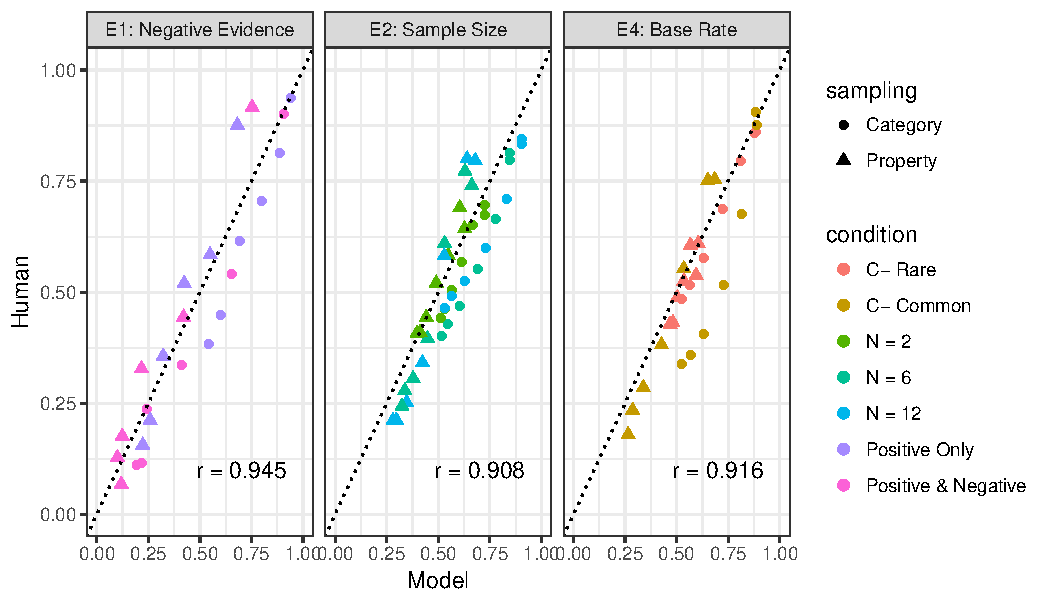
\includegraphics{./fits_scatter.pdf}
\caption{Model selection as viewed as a statistical problem typically emphasises quantitative measures of agreement between model predictions (or fitted values, x-axis) and human responses (y-axis). Even without any explanation given for the condition names or the experimental design, it is clear that the model in this figure provides a very good fit to the data. Nevertheless, knowing that the model fits depend on the values of parameters estimated from data, one might be tempted to ask if the researcher has encountered the Scylla of overfitting. Perhaps this apparent good performance is an illusion.}
\end{figure}

Gronau and Wagenmakers (2018) frame the question of model selection as a
perilous dilemma in which one is caught between two beasts from
classical mythology, the \emph{Scylla} of overfitting and the
\emph{Charybdis} of underfitting. I find myself often on the horns of a
quite different dilemma, namely the tension between the \emph{devil} of
statistical decision making and the \emph{deep blue sea} of addressing
scientific questions. If I have any strong opinion at all on this topic,
it is that much of the model selection literature places too much
emphasis on the statistical issues of model choice and too little on the
scientific questions to which they attach.

To again focus on my own papers rather than criticise others, consider
the model fits reported by Hayes, Banner, Forrester and Navarro (under
review). In that paper we were interested in how people's inductive
reasoning from data is shaped by what they know about the process by
which the data were selected, referred to as \emph{sensitivity to
sampling} in the literature. This is a theme I have explored across
multiple papers in the last several years. To model sensitivity to
sampling we relied on earlier work by Tenenbaum and Griffiths (2001), as
do most papers I have written on this topic (e.g., Navarro, Dry \& Lee
2012, Ransom, Perfors \& Navarro 2016, Voorspoels, Navarro, Perfors,
Ransom \& Storms, 2015). However, the task that we used in the Hayes et
al. (under review) paper differs from previous ones in many ancillary
respects, and these ancillary details need to be formalised in specific
model choices. Some such choices (e.g., how smooth is an unknown
generalisation function?) can be instantiated as model parameters, but
others (e.g., what class of functions is admissable to describe human
generalisation?) are not so simple. I think the choices I made are
sensible, but reasonable people might disagree.

How should I evaluate my modelling choices? A statistical perspective on
this inference problem might begin by estimating model parameters
\(\theta\) and producing a measure of predictive performance. Setting
aside the computational details of how one does this, the result is
likely to lead to a comparison between model predictions and human
performance similar to the one shown in Figure 1. Even without knowing
the particular details of the experiments, the scatterplot showing the
fitted model values (x-axis) against the average reponse given by human
participants (y-axis) across a large number of experimental conditions
strongly suggests that the model fits the empirical data well.

Perhaps it fits too well? When presented with such a figure, a reader
familiar with the model selection literature might be concerned that I
have run afoul of the Scylla of overfitting. This is not an unreasonable
concern, but I find myself at a loss as to how cross-validation, Bayes
factors, or any other automated method can answer it. My scientific goal
when constructing this model was \emph{not} to maximise the correlations
as shown in Figure 1, it was to \emph{make sense} of the observed
generalisation curves shown in Figure 2. The data in Figure 2 are the
same as those plotted in Figure 1, but drawn in a way that highlights
the empirical effects of theoretical interest. In each column there are
multiple generalisation curves shown, plotted separately for each
experimental condition, with human data at the top and model predictions
at the bottom. It is clear from inspection that the data are highly
structured, and that there are systematic patterns to how people's
judgements change across conditions. The scientific question of most
interest to me is asking what theoretical principles are required to
produce these shifts. Providing a good fit to the data seems of
secondary importance. From visual inspection it is clear that the model
captures \emph{most} patterns in the data, but not all. In particular,
looking at the systematic model failure in the second column from the
right, the same reader might now be inclined to wonder if I have fallen
prey to the Charybdis of \emph{underfitting}. So which of the mythical
beasts, Scylla or Charybdis, have I encountered? Would a
cross-validation analysis or Bayes factor calculation tell me? It seems
unlikely.

\begin{figure}
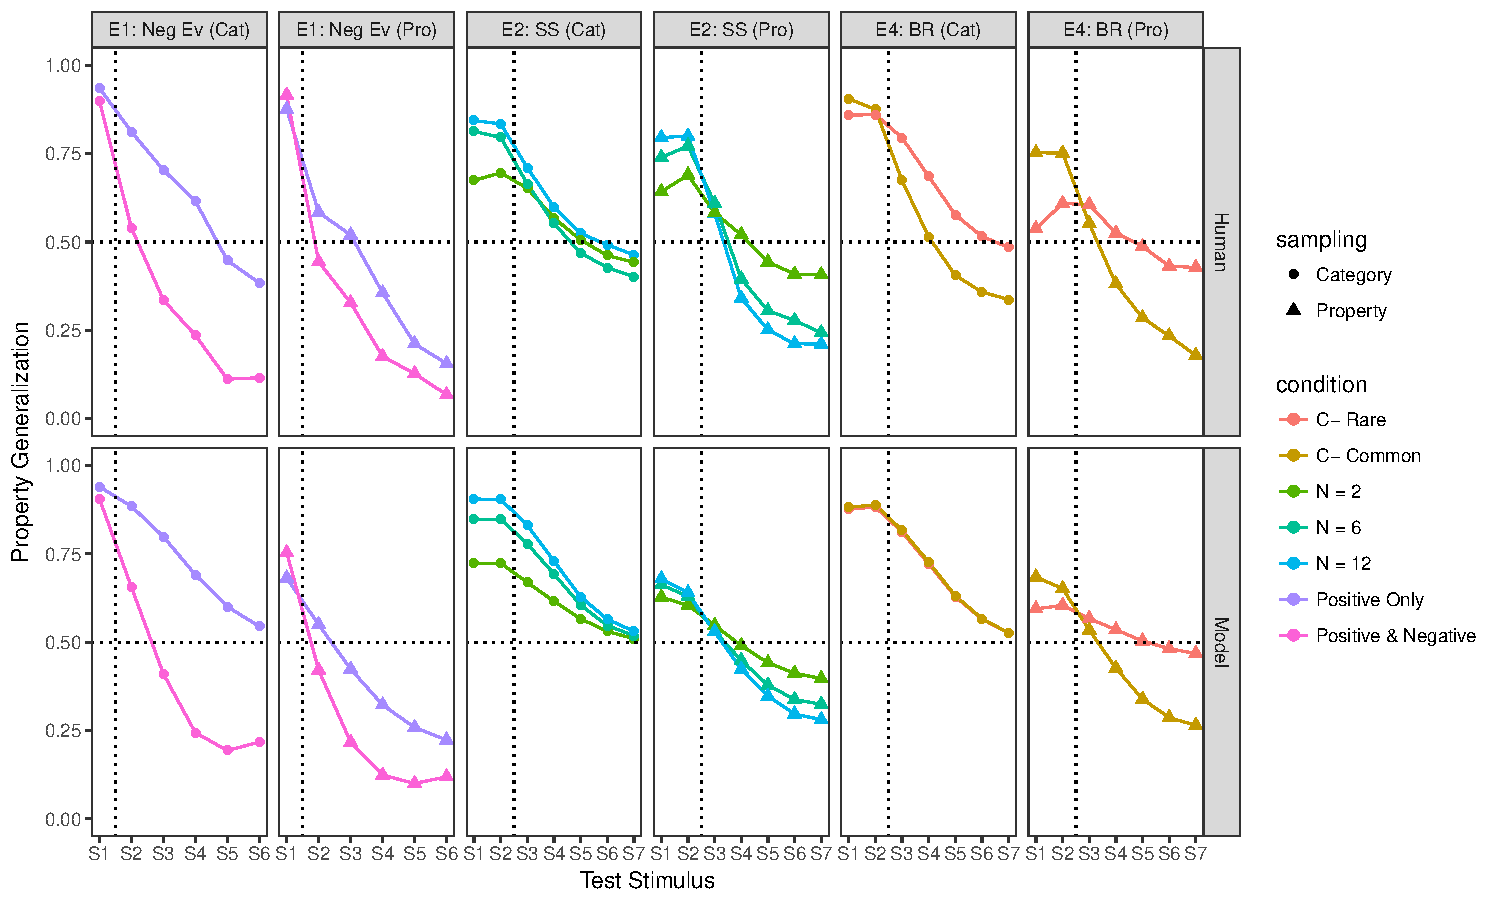
\includegraphics{./fits_line.pdf}
\caption{Scientific model selection is often more concerned with making sense of the systematic patterns observed in empirical data. This plots depict the extent to which people (top row) or a model (bottom row) will generalise (y-axis) from a small sample of training data to a novel item, shown as a function of the similarity of the novel item (x-asis) to the training data, with the most similar items shown on the left. Different panels (columns) and curves plotted separately as a function of three different experimental conditions reported by Hayes et al (under review). Even without a clear explanation of the different manipulations and their theoretical import, it is clear that the model provides a good account of the data in most conditions, but notably cannot reproduce the effect shown in the second panel from the right. One may be led to wonder if the researcher has encountered the Charybdis of underfitting. (Note: the data and model are the same as those plotted in Figure 1)}
\end{figure}

To my mind, the bigger concern here is that to focus too heavily on the
issue of under/overfitting is to be seduced by the devil of statistical
decision making. When we actually analysed the data, the allure of the
deep blue sea of science led us to a different perspective. The approach
we took was to ignore the quantitative fits almost entirely, and focus
on the extent to which the key \emph{qualitative} patterns in the data
are an invariant prediction of the model across different choices of the
parameter values \(\theta\). Loosely inspired by the \enquote{parameter
space partitioning} idea introduced by Pitt, Kim, Navarro and Myung
(2006), we defined a set of ordinal constraints in the data that any
theoretical account would need to explain (e.g., increasing the number
of observations caused a crossover effect under property sampling,
column 4 from the left), and then showed that under most parameter
values in the model, the predictions about these ordinal effects did not
change. In other words -- to recast this in the \enquote{scientific
versus technological} language used by Bernardo and Smith (2000) -- the
scientifically important patterns are captured by
\(P(\bm{x}|\theta, \mathcal{M})\) regardless of the specific value of
\(\theta\).

To my way of thinking, understanding how the qualitative patterns in the
empirical data emerge naturally from a computational model of a
psychological process is often more scientifically useful than
presenting a quantified measure of its performance, but it is the latter
that we focus on in the \enquote{model selection} literature. Given how
little psychologists understand about the varied ways in which human
cognition works, and given the artificiality of most experimental
studies, I often wonder what purpose is served by quantifying a model's
ability to make precise predictions about every detail in the data. Much
as the false confidence of the Bayes factor in the \enquote{negligible
error} scenario I constructed at the beginning is entirely an artifact
of its sensitivity to a bad ancillary assumption made by one of the
models (that \(\theta\) must be exactly 1 for a general law to hold), it
seems to me that in real life, many exercises in which model choice
relies too heavily on quantitative measures of performance are
essentially selecting models based on their ancillary assumptions. It is
unclear to me if this solves a scientific problem of interest.

\section{References}\label{references}

\begingroup
\setlength{\parindent}{-0.5in} \setlength{\leftskip}{0.5in}

Akaike, H. (1973). Information theory and an extension of the maximum
likelihood principle. In B. N. Petrov \& F. Csaki (eds), \emph{Second
International Symposium on Information Theory}, pp.~267-281. Budapest:
Akademiai Kiado.

Bernardo, J. M. \& Smith, A. F. M. (2000). \emph{Bayesian Theory} (2nd
edition). John Wiley \& Sons.

Box, G. E. P. (1976). Science and statistics. \emph{Journal of the
American Statistical Association, 71}, 791-799.

Browne, M. (2000). Cross-validation methods. \emph{Journal of
Mathematical Psychology, 44}, 108-132.

Devezer, B., Nardin, L. G., Baumgaertner, B. \& Buzbas, E. (under
review). Discovery of truth is not implied by reproducibility but
facilitated by innovation and epistemic diversity in a model-centric
framework. \emph{Manuscript submitted for publication}.
arxiv.org/abs/1803.10118

Edwards, W., Lindman, H. \& Savage, L. J. (1963). Bayesian statistical
inference for psychological research. \emph{Psychological Review, 70},
193-242.

Gelman, A., Carlin, J. B., Stern, H. S., \& Rubin, D. B. (2003).
\emph{Bayesian Data Analysis} (2nd ed)

Grünwald, P. (2007). \emph{The minimum description length principle}.
Cambridge, MA: MIT Press.

Gronau, Q. \& Wagenmakers, E. J. (2018). Limitations of Bayesian
leave-one-out cross-validation for model selection.

Hayes, B.K., Banner, S., Forrester, S. \& Navarro, D.J. (under review).
Sampling frames and inductive inference with censored evidence.
\emph{Manuscript submitted for publication}.
\url{https://doi.org/10.17605/OSF.IO/2M83V}

Kamin, L.J. (1969). Predictability, surprise, attention, and
conditioning. In B. A. Campbell and R. M. Church (Eds.) \emph{Punishment
and Aversive Behavior}. New York: Appleton-Century-Crofts (pp 279-296).

Kruschke, J. K. (1992). ALCOVE: An exemplar-based connectionist model of
category learning. \emph{Psychological Review, 99}(1), 22-44.

Lake, B. M., Salakhutdinov, R. \& Tenenbaum, J. B. (2015). Human-level
concept learning through probabilistic program induction. \emph{Science,
350}(6266), 1332-1338.

Lattal, K. M., \& Nakajima, S. (1998). Overexpectation in appetitive
Pavlovian and instrumental conditioning. \emph{Animal Learning \&
Behavior, 26}(3), 351-360.

Lee, M. D. (2001a). On the complexity of additive clustering models.
\emph{Journal of Mathematical Psychology, 45}, 131-148.

Lee, M. D. (2001b). Determining the dimensionality of multidimensional
scaling models for cognitive modeling. \emph{Journal of Mathematical
Psychology, 45}, 149-166.

Lee, M. D. \& Navarro, D. J. (2002). Extending the ALCOVE model of
category learning to featural stimulus domains \emph{Psychonomic
Bulletin \& Review, 9}, 43-58

Navarro, D. J. (2004). A note on the applied use of MDL approximations.
\emph{Neural Computation, 16}, 1763-1768

Navarro, D. J., Dry, M. J. \& Lee, M. D. (2012). Sampling assumptions in
inductive generalization. \emph{Cognitive Science, 36}, 187-223

Navarro, D. J., Pitt M. A. \& Myung, I. J. (2004). Assessing the
distinguishability of models and the informativeness of data.
\emph{Cognitive Psychology, 49}, 47-84

Pavlov, I. (1927). \emph{Conditioned Reflexes}. London: Oxford
University Press

Pitt, M. A., Myung, I. J. \& Zhang, S. (2002). Toward a method of
selecting among computational models of cognition. \emph{Psychological
Review, 109}, 472-491.

Pitt, M. A., Kim, W., Navarro, D. J. \& Myung, J. I. (2006). Global
model analysis by parameter space partitioning. \emph{Psychological
Review, 113}, 57-83.

Rescorla, R. A. (1968). Probability of shock in the presence and absence
of CS in fear conditioning. \emph{Journal of Comparative and
Physiological Psychology, 66}, 1-5.

Rescorla, R.A. (1969) Conditioned inhibition of fear resulting from
negative CS-US contingencies. \emph{Journal of Comparative and
Physiological Psychology, 67}, 504-509.

Rescorla, R. A. (1971) Variations in the effectiveness of reinforcement
following prior inhibitory conditioning. \emph{Learning and Motivation,
2}, 113-123.

Rescorla, R. A. \& Wagner, A. R. (1972) A theory of Pavlovian
conditioning: Variations in the effectiveness of reinforcement and
nonreinforcement. In A. H. Black \& W. F. Prokasy (eds) \emph{Classical
conditioning II: Current Research and Theory} (pp 64-99). New York:
Appleton-Century-Crofts

Ransom, K., Perfors, A. \& Navarro, D. J. (2016). Leaping to
conclusions: Why premise relevance affects argument strength.
\emph{Cognitive Science, 40}, 1775-1796

Rissanen, J. (1996). Fisher information and stochastic complexity.
\emph{IEEE Transactions on Information Theory 42}, 40-47.

Schultz, W., Dayan, P., \& Montague, P. R. (1997). A neural substrate of
prediction and reward. \emph{Science, 275}(5306), 1593-1599.

Schwarz, G. (1978). Estimating the dimension of a model. \emph{The
Annals of Statistics, 6}, 461-464

Shao, J. (1993). Linear model selection by cross-validation.
\emph{Journal of the American Statistical Association 88}, 486-494.

Shiffrin, R. M., Borner, K. \& Stigler, S. M. (2018). Scientific
progress despite irreproducibility: A seeming paradox. \emph{Proceedings
of the National Academy of Sciences, USA}, 115, 2632-2639.

Tenenbaum, J. B. \& Griffiths, T. L. (2001). Generalization, similarity,
and Bayesian inference. \emph{Behavioral and Brain Sciences, 24},
629-640.

Vehtari, A., Simpson, D., Yao, Y. \& Gelman, A. (2018). Limitations of
\enquote{Limitations of Bayesian leave-one-out cross-validation}

Vehtari, A. \& Ojanen, J. (2012). A survey of Bayesian predictive
methods for model assessment, selection and comparison. \emph{Statistics
Surveys 6}, 142-228.

Voorspoels, W., Navarro, D. J., Perfors, A., Ransom, K. \& Storms, G.
(2015). How do people learn from negative evidence? Non-monotonic
generalizations and sampling assumptions in inductive reasoning.
\emph{Cognitive Psychology, 81}, 1-25

Wickelgren, W. A. (1972). Trace resistance and decay of long-term
memory. \emph{Journal of Mathematical Psychology, 9}, 418-455.

\endgroup


\end{document}
